\documentclass[14pt]{extbook}
\usepackage{multicol, enumerate, enumitem, hyperref, color, soul, setspace, parskip, fancyhdr} %General Packages
\usepackage{amssymb, amsthm, amsmath, bbm, latexsym, units, mathtools} %Math Packages
\everymath{\displaystyle} %All math in Display Style
% Packages with additional options
\usepackage[headsep=0.5cm,headheight=12pt, left=1 in,right= 1 in,top= 1 in,bottom= 1 in]{geometry}
\usepackage[usenames,dvipsnames]{xcolor}
\usepackage{dashrule}  % Package to use the command below to create lines between items
\newcommand{\litem}[1]{\item#1\hspace*{-1cm}\rule{\textwidth}{0.4pt}}
\pagestyle{fancy}
\lhead{Progress Quiz 5}
\chead{}
\rhead{Version A}
\lfoot{9912-2038}
\cfoot{}
\rfoot{Spring 2021}
\begin{document}

\begin{enumerate}
\litem{
Determine the domain of the function below.\[ f(x) = \frac{6}{9x^{2} +6 x -15} \]\begin{enumerate}[label=\Alph*.]
\item \( \text{All Real numbers except } x = a, \text{ where } a \in [-1.9, -1] \)
\item \( \text{All Real numbers.} \)
\item \( \text{All Real numbers except } x = a \text{ and } x = b, \text{ where } a \in [-1.9, -1] \text{ and } b \in [0.6, 1.8] \)
\item \( \text{All Real numbers except } x = a \text{ and } x = b, \text{ where } a \in [-16.3, -14.1] \text{ and } b \in [8.4, 9.6] \)
\item \( \text{All Real numbers except } x = a, \text{ where } a \in [-16.3, -14.1] \)

\end{enumerate} }
\litem{
Choose the graph of the equation below.\[ f(x) = \frac{1}{x + 1} - 2 \]\begin{enumerate}[label=\Alph*.]
\begin{multicols}{2}\item 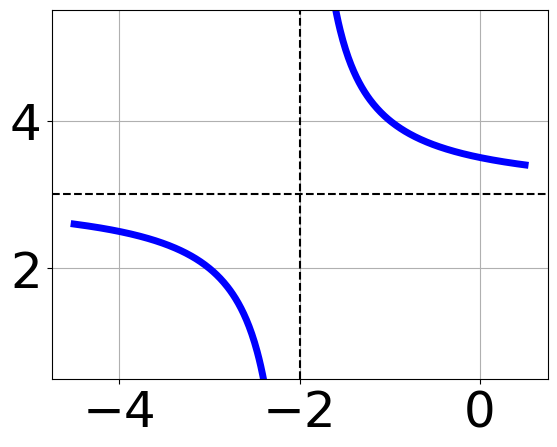
\includegraphics[width = 0.3\textwidth]{../Figures/rationalEquationToGraphCopyAA.png}\item 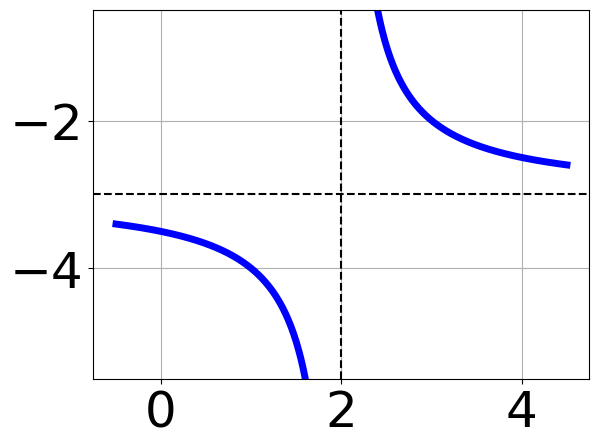
\includegraphics[width = 0.3\textwidth]{../Figures/rationalEquationToGraphCopyBA.png}\item 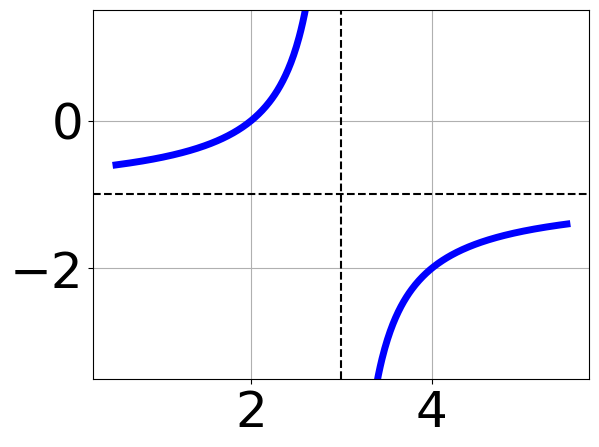
\includegraphics[width = 0.3\textwidth]{../Figures/rationalEquationToGraphCopyCA.png}\item 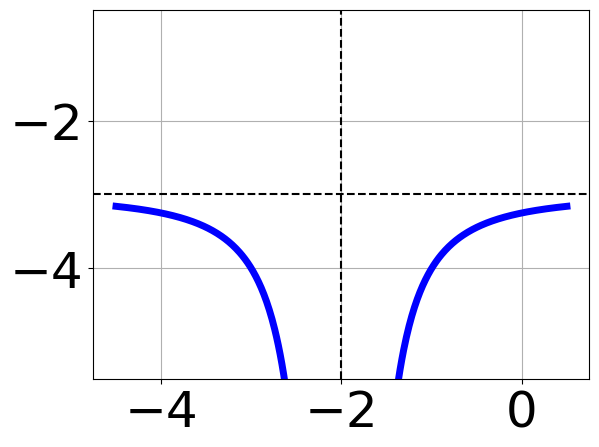
\includegraphics[width = 0.3\textwidth]{../Figures/rationalEquationToGraphCopyDA.png}\end{multicols}\item None of the above.
\end{enumerate} }
\litem{
Choose the equation of the function graphed below.
\begin{center}
    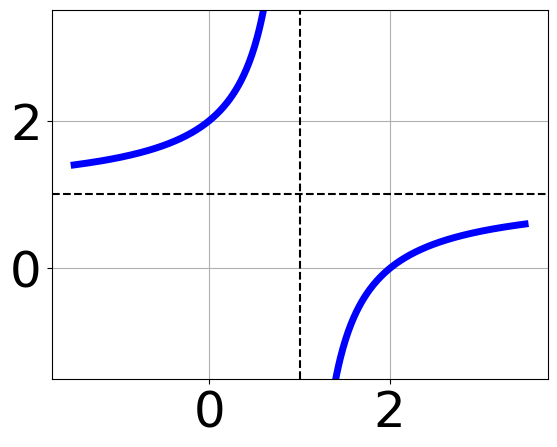
\includegraphics[width=0.5\textwidth]{../Figures/rationalGraphToEquationCopyA.png}
\end{center}
\begin{enumerate}[label=\Alph*.]
\item \( f(x) = \frac{1}{(x + 3)^2} - 2 \)
\item \( f(x) = \frac{-1}{(x - 3)^2} - 2 \)
\item \( f(x) = \frac{1}{x + 3} - 2 \)
\item \( f(x) = \frac{-1}{x - 3} - 2 \)
\item \( \text{None of the above} \)

\end{enumerate} }
\litem{
Choose the graph of the equation below.\[ f(x) = \frac{-1}{(x + 2)^2} - 2 \]\begin{enumerate}[label=\Alph*.]
\begin{multicols}{2}\item 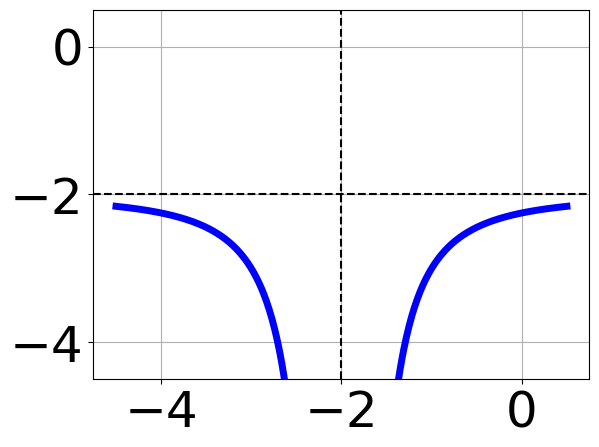
\includegraphics[width = 0.3\textwidth]{../Figures/rationalEquationToGraphAA.png}\item 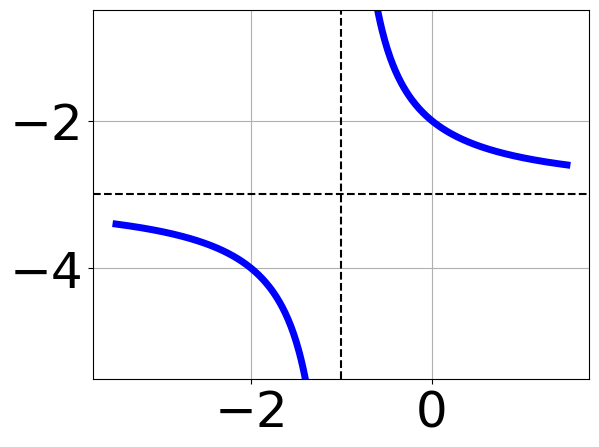
\includegraphics[width = 0.3\textwidth]{../Figures/rationalEquationToGraphBA.png}\item 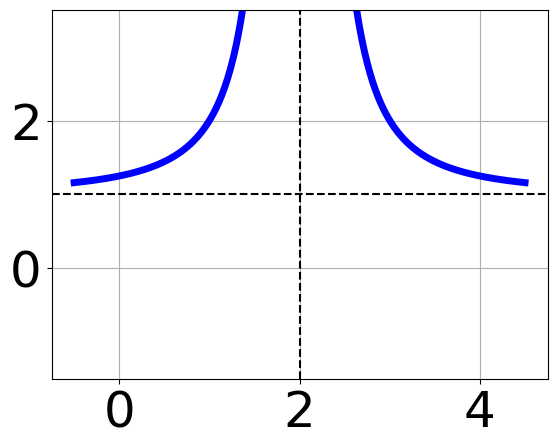
\includegraphics[width = 0.3\textwidth]{../Figures/rationalEquationToGraphCA.png}\item 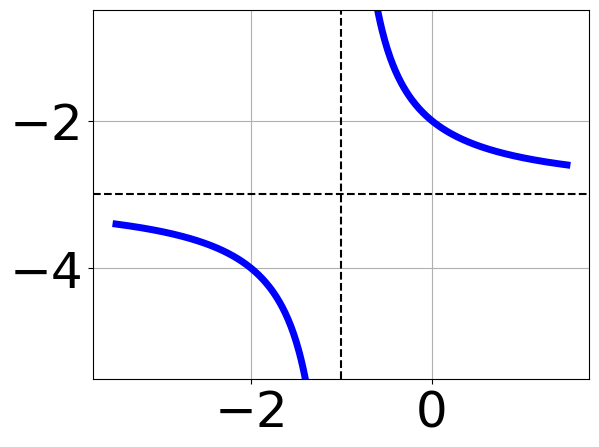
\includegraphics[width = 0.3\textwidth]{../Figures/rationalEquationToGraphDA.png}\end{multicols}\item None of the above.
\end{enumerate} }
\litem{
Solve the rational equation below. Then, choose the interval(s) that the solution(s) belongs to.\[ \frac{3}{-4x + 7} + -7 = \frac{-3}{-20x + 35} \]\begin{enumerate}[label=\Alph*.]
\item \( x \in [1.62,2.62] \)
\item \( x_1 \in [-1.94, -1.82] \text{ and } x_2 \in [1.62,3.62] \)
\item \( x_1 \in [1.49, 1.62] \text{ and } x_2 \in [1.62,3.62] \)
\item \( x \in [-1.94,-1.82] \)
\item \( \text{All solutions lead to invalid or complex values in the equation.} \)

\end{enumerate} }
\litem{
Solve the rational equation below. Then, choose the interval(s) that the solution(s) belongs to.\[ \frac{-6x}{-7x -3} + \frac{-5x^{2}}{42x^{2} -24 x -18} = \frac{-4}{-6x + 6} \]\begin{enumerate}[label=\Alph*.]
\item \( x_1 \in [-0.94, 0.1] \text{ and } x_2 \in [0.2,3.1] \)
\item \( x \in [0.59,1.17] \)
\item \( x_1 \in [-0.94, 0.1] \text{ and } x_2 \in [-2.5,0.8] \)
\item \( x \in [1.58,2.73] \)
\item \( \text{All solutions lead to invalid or complex values in the equation.} \)

\end{enumerate} }
\litem{
Determine the domain of the function below.\[ f(x) = \frac{6}{15x^{2} +48 x + 36} \]\begin{enumerate}[label=\Alph*.]
\item \( \text{All Real numbers except } x = a \text{ and } x = b, \text{ where } a \in [-2.81, -1.6] \text{ and } b \in [-1.38, -0.99] \)
\item \( \text{All Real numbers except } x = a, \text{ where } a \in [-2.81, -1.6] \)
\item \( \text{All Real numbers except } x = a \text{ and } x = b, \text{ where } a \in [-30.07, -29.63] \text{ and } b \in [-18.33, -17.26] \)
\item \( \text{All Real numbers except } x = a, \text{ where } a \in [-30.07, -29.63] \)
\item \( \text{All Real numbers.} \)

\end{enumerate} }
\litem{
Solve the rational equation below. Then, choose the interval(s) that the solution(s) belongs to.\[ \frac{7}{-7x + 2} + -4 = \frac{2}{14x -4} \]\begin{enumerate}[label=\Alph*.]
\item \( x \in [-1.07,-0.45] \)
\item \( x \in [-1.0,1.0] \)
\item \( x_1 \in [-1.07, -0.45] \text{ and } x_2 \in [-0.24,0.04] \)
\item \( x_1 \in [-0.52, 0.2] \text{ and } x_2 \in [0.08,0.19] \)
\item \( \text{All solutions lead to invalid or complex values in the equation.} \)

\end{enumerate} }
\litem{
Solve the rational equation below. Then, choose the interval(s) that the solution(s) belongs to.\[ \frac{5x}{3x -5} + \frac{-6x^{2}}{-9x^{2} -3 x + 30} = \frac{4}{-3x -6} \]\begin{enumerate}[label=\Alph*.]
\item \( \text{All solutions lead to invalid or complex values in the equation.} \)
\item \( x \in [-2.3,-1.44] \)
\item \( x_1 \in [-0.36, 1.22] \text{ and } x_2 \in [-0.33,2.67] \)
\item \( x \in [-3.05,-2.04] \)
\item \( x_1 \in [-0.36, 1.22] \text{ and } x_2 \in [-4.4,1.6] \)

\end{enumerate} }
\litem{
Choose the equation of the function graphed below.
\begin{center}
    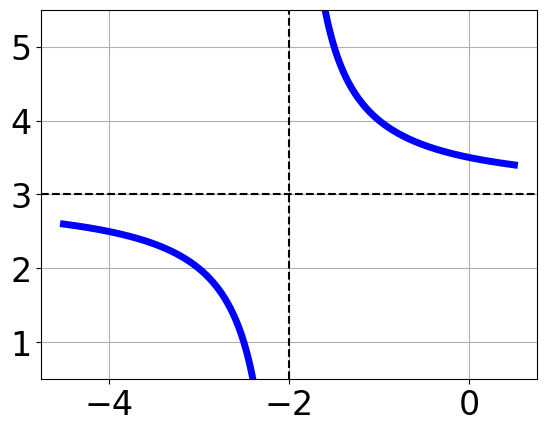
\includegraphics[width=0.5\textwidth]{../Figures/rationalGraphToEquationA.png}
\end{center}
\begin{enumerate}[label=\Alph*.]
\item \( f(x) = \frac{1}{(x - 1)^2} + 3 \)
\item \( f(x) = \frac{-1}{(x + 1)^2} + 3 \)
\item \( f(x) = \frac{-1}{x + 1} + 3 \)
\item \( f(x) = \frac{1}{x - 1} + 3 \)
\item \( \text{None of the above} \)

\end{enumerate} }
\end{enumerate}

\end{document}